\documentclass{article}
\usepackage{graphicx} % Required for inserting images
\usepackage[margin=1in]{geometry}
\usepackage{amsmath}
\usepackage{amsthm}
\usepackage{amssymb}
\usepackage{amsfonts}
\usepackage{verbatim}
\usepackage{xcolor}

\title{Homework 3: Report}
\author{Dante Buhl}
\date{Feb. $14^{th}$ 2024}

\begin{document}

\newcommand{\bs}[1]{\boldsymbol{#1}}
\newcommand{\bmp}[1]{\begin{minipage}{#1\textwidth}}
\newcommand{\emp}{\end{minipage}}
\newcommand{\R}{\mathbb{R}}
\newcommand{\C}{\mathbb{C}}
\newcommand{\N}{\mathcal{N}}
\newcommand{\I}{\mathrm{I}}
\newcommand{\K}{\bs{\mathrm{K}}}
\newcommand{\m}{\bs{\mu}_*}
\newcommand{\s}{\bs{\Sigma}_*}
\newcommand{\dt}{\Delta t}
\newcommand{\tr}[1]{\text{Tr}(#1)}
\newcommand{\Tr}[1]{\text{Tr}(#1)}

\maketitle

\colorbox{yellow}{All example code outputs are in stored in a text file, ``output.txt'', within the fortran tar-ball.}

\section{Warming-Up Fortran Routines}
\begin{enumerate}
\item Write a function which computes the trace of a square matrix A. 

This was not all too difficult, in fact it only used one loop. On first inspection it also seems to be accurally calculating the trace of matrix A from Amat.dat. 

\item Write a function which computes the two norm of a (column) vector.

This was also not very difficult, besides defining my variables, this took 1 line of code. 

\item Write a function which prints a matrix and its dimensions to a screen.

This was slightly more complex, in that I like to format my print statements in fortran for matrices. So I chose an arbitrary amount of digits to keep and added a small routine for turning integers in string formats.

\item Write a driver routine which reads in a matrix from Amat, and then computes its trace, prints it to the terminal, and then computes the norm of each of its column vectors. 

This was very simple. I decided to use one driver file for all 3 of the main programing questions. I simply called the routines from my module, and made sure to use all of the routines I had placed in my module at the top of the file. 

\begin{center}
    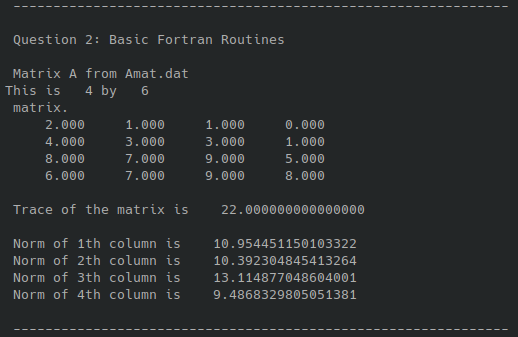
\includegraphics[width = .6\textwidth]{files/Q2sol.png}
\end{center}

\end{enumerate}

\section{Gaussian Elimination with Pivoting}
\begin{enumerate}
\item Write a subroutine which performs Gaussian Elimination with Pivoting to on a Matrix A and a rhs-matrix B. 

This was tricky and I realized about midway through that storing the permutation matrix was a little crazy (especially for very large scale problems which I don't necessarily have to care about right now). So I changed the method I was pivoting and now it seems to work very well. 

\item Write a subroutine which performs backsubstitution to solve the linear system $UX = B$. 

This was a fairly short routine and not very difficult. It can be easily scaled so that it computes the solutions for all columns of B at once, so I programmed it to do so. 

\item Write a driver routine which calls your GE subroutine and backsub subroutine, and prints the matrices, before GE, after GE but before backsubstitution, the solution matrix X, and the error matrix $E = B_s - A_sX$, and the 2-norms of the column vectors of $E$. 

The code runs very well except for the fact that there is a small artifact of error for the one very odd, 5th column of B in Bmat.dat. The error for that specific column in of order $10^{-13}$ rather than $10^{-16}$ which we all know and love to be machine double precision. I'm going to double check the backsub routine to see if there is any large gleaming issue with it (I've triple checked the GE and LU routines and there is no error there). Below is the found solution and error.

\begin{center}
    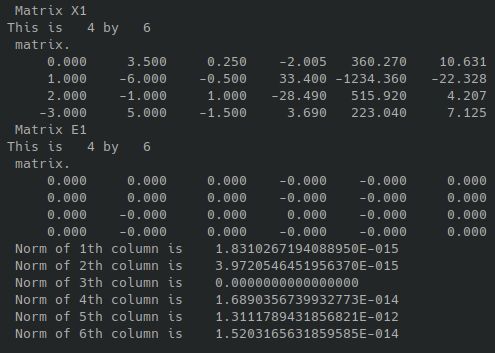
\includegraphics[width = .6\textwidth]{files/GEsol.png}
\end{center}

\end{enumerate}

\section{LU Decomposition with Pivoting}
\begin{enumerate}
\item Write a subroutine which performs LU Decomposition with Pivoting to on a Matrix A. 

This routine was very similar to my GE routine except that it doesn't do any computations for the matrix B. The permutation matrix was also very easy to return. I did the actual calculation manually and found the same matrices that my decomposition yields. 

\item Write a subroutine which performs forward subsitution and backwards substitution to solve the linear system $UX = Y$, $LY = B$ for $X$. 

This was also very straight forward and easily scalable for rhs matrices. I used the same backsub routine from GE to solve, $UX = Y$ and wrote a forward subroutine to solve $LY = PB$. 

\item Write a driver routine which calls your LU subroutine and LU solver routine, and prints A before LU decompition, A, L, and U after the decomposition, the solution matrix X after solving, and the error matrix $E = B_s - A_sX$, and the 2-norms of the column vectors of $E$. 

This method goes as planned and has the same exact solution you find in GE. With nearly the same error norms as in GE. It has the same artifact of error as the GE method. 

\begin{center}
    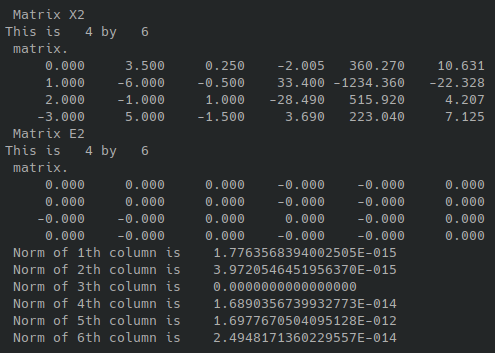
\includegraphics[width = .6\textwidth]{files/LUsol.png}
\end{center}

\end{enumerate}

\section{Theory Problems}
\begin{enumerate}

\item %start of problem 1
The Schur decomposition theorem states that if $A \in C^{m\times m}$, then there
exist a unitary matrix $Q$ and an upper triangular matrix $U$ such that
$A = QUQ^{-1}$ . Use the Schur decomposition theorem to show that a real
symmetric matrix $A$ is diagonalizable by an orthogonal matrix, i.e., $\exists$ an
orthogonal matrix $Q$ such that $Q^T AQ = D$, where $D$ is a diagonal matrix
with its eigenvalues in the diagonal.

\begin{proof}

We begin with the Schur Decomposition Theorm for real symmetric matrix $A$. We have, 
\[
    A = QUQ^{-1} = QUQ^*
\]
By the property that $A$ is real and symmetric, we have that $A^* = A$.
\[
    A^* = A = QUQ^*
\]
\[
    Q^*A^*Q = U^* = Q^*AQ = U
\]
So we have, $U = U^*$. Since we have that $U$ is upper triangular, that means that $U^*$ is lower triangular. However, since they are equal to one another, we must have that they are both diagonal. Thereby we have that $A$ is diagonalizable by an othorgonal matrix $Q$ (a property of unitary matrices).
\[
    A = QUQ^* \implies Q^{-1}AQ = U = D
\]
Since we have this property, we have that $Q$ contains the eigenvectors of $A$ and $U$ is a diagonal matrix contianing its eigenvalues. 

\end{proof}

\item
Consider the following system
\[
\left(\begin{array}{c c}
1 & 1 \\
\epsilon & 1 
\end{array}\right) \left(\begin{array}{c}
x \\
y
\end{array}\right) = \left(\begin{array}{c}
2 \\ 
1
\end{array}\right) 
\]
Multiply the last row of the matrix and the right-hand side vector by a large
constant $c$ such that $c\epsilon \gg 1$. Perform Gaussian elimination with partial
pivoting to the modified row-scaled system and discuss what happens. If
solving the resulting system has numerical issues, identify the issues and
discuss how to improve the method.

\[
\left(\begin{array}{c c}
1 & 1 \\
c\epsilon & c 
\end{array}\right) \left(\begin{array}{c}
x \\
y
\end{array}\right) = \left(\begin{array}{c}
2 \\ 
c
\end{array}\right) 
\]
\[
\left(\begin{array}{c c}
1 & 1 \\
0 & c(1-\epsilon) 
\end{array}\right) \left(\begin{array}{c}
x \\
y
\end{array}\right) = \left(\begin{array}{c}
2 \\ 
c(1-2\epsilon)
\end{array}\right) 
\]
\[
    y = \frac{1 - 2\epsilon}{1 - \epsilon} \approx 1
\]
\[
    x = \frac{1}{1- \epsilon} \approx 1
\]
This method actually does a decent job computing $x$ and $y$ within machine precision.

\item   What can you say about the diagonal entries of a symmetric positive definite matrix? Justify your assertion.

Claim: All diagonal entries of a symmetric pos. def. matrix are positive. 

\begin{proof}
    Take $A$ to be a symmetric positive definite square matrix, $A \in \C^{m\times m}$. We have that for all vectors $x \in \C^m$, that the inner product is greater than zero, (.i.e. $(x, Ax) > 0$). We can now chose vectors $x$ to demonstrate that the diagonal elements are positive. Let us chose $x = \hat{e}_1$.
\[
    (\hat{e}_1, A\hat{e}_1) = \hat{e}_1^*A\hat{e}_1 = \hat{e}_1^*\vec{a}_1
\]
Where $\vec{a}_i$ is the ith column vector of $A$. 
\[
    (\hat{e}_1, A\hat{e}_1) = \hat{e}_1^*\vec{a}_1 = a_{11} 
\]
\[
      (\hat{e}_1, A\hat{e}_1) > 0 \implies a_{11} > 0
\]
This argument can be repeated for unit basis vectors, $\hat{e}_i, \forall i \in 1, \cdots, m$. Thus we have, that $a_{ii} > 0 \forall i \in 1, \cdots, m$.
\end{proof}


\item Suppose $A \in \C^{m \times m}$ is written in the block form
\[
A = \left(\begin{array}{c c}
        A_{11} & A_{12}\\
        A_{21} & A_{22}
    \end{array}\right)
\]
where $A_{11} \in \C^{n\times n}$ and $A_{22} \in \C^{(m-n)\times(m-n)}$. Assume that A satisfies the condition: $A$ has an $LU$ decomposition if and only if the upper-left $k\times k$ block matrix $A_{1:k,1:k}$ is nonsingular for each $k$ with $1 \le k \le m$.
\begin{enumerate}
\item Verify the formula
\[
 \left(\begin{array}{c c}
        \I & 0\\
        -A_{21}A_{11}^{-1} & \I
    \end{array}\right)
 \left(\begin{array}{c c}
        A_{11} & A_{12}\\
        A_{21} & A_{22}
    \end{array}\right) =  \left(\begin{array}{c c}
        A_{11} & A_{12}\\
        0 & A_{22} - A_{21}A_{11}^{-1}A_{12}
    \end{array}\right)
\]
which “eliminate” the block $A_{21}$ from $A$. The matrix $A_{22}-A_{21}A_{11}^{-1}A_{12}$ is known as the Schur complement of $A_{11}$ in $A$, denoted as $A/A_{11}$.

\begin{proof}

\[
 \left(\begin{array}{c c}
        \I & 0\\
        -A_{21}A_{11}^{-1} & \I
    \end{array}\right)
 \left(\begin{array}{c c}
        A_{11} & A_{12}\\
        A_{21} & A_{22}
    \end{array}\right) =  \left(\begin{array}{c c}
        \I A_{11} & \I A_{12}\\
        \I A_{21} - A_{21}A_{11}^{-1}A_{11} & \I A_{22} - A_{21}A_{11}^{-1}A_{12}
    \end{array}\right)
\]
\[
    =  \left(\begin{array}{c c}
            A_{11} & A_{12}\\
            A_{21} - A_{21} & A_{22} - A_{21}A_{11}^{-1}A_{12}
        \end{array}\right) =  \left(\begin{array}{c c}
            A_{11} & A_{12}\\
            0  & A_{22} - A_{21}A_{11}^{-1}A_{12}
        \end{array}\right) 
\]

\end{proof}

\item Suppose that after applying n steps of Gaussian elimination on the
matrix $A$ in (2), $A_{21}$ is eliminated row by row, resulting in a matrix
\[
    \left(\begin{array}{c c}
        A_{11} & C\\
        0 & D
    \end{array}\right)
\]
Show that the bottom-right $(m -n)\times(m-n)$ block matrix $D$ is
again $A_{22} - A_{21}A_{11}^{-1}A_{12}$. Note: Part (b) is separate from Part (a)).
\begin{proof}
We start by looking at the process of gaussian elimination. We have that we progress by devloping these $L$ matrices, so as to eliminate the entries below the diagonal element in each column. We look at $L_1$. 
\[
    L_1 = \left(\begin{array}{c c c c}
            1 & 0 & \cdots & \textbf{0} \\
            -\frac{a_{21}}{a_{11}} & \ddots & \cdots & \textbf{0} \\
            \vdots & 0  & \ddots & \textbf{0}\\
            -\frac{\vec{a_{21}}^1}{a_{11}} & \vdots & \cdots & \I
            \end{array}\right)
\]
Where $\vec{a_{21}}^i$ denotes the ith column vector of $A_{21}$. 
We will ultimately have,
\[
    D(i, j) = A_{22}(i, j) - \sum_{k=1}^{n}\frac{1}{a_{kk}}(\vec{a_{21}}^k(i) \cdot \vec{a_{12}}^k(j))
\]
with $a_{kk}$ are the diagonal elements of $A_{11}$, and $\vec{a_{12}}^k$ is the kth column vector of $A_{12}$.
Note that if $A_{11}$ is a diagonal block matrix, then this exactly gives, 
\[
    D = A_{22} - A_{21}A_{11}^{-1}A_{12}
\]


\end{proof}
\end{enumerate}

\item Consider solving $Ax = b$, with $A$ and $b$ are complex-valued of order $m$, i.e., $A \in \C^{m\times m}, b \in \C^m$.
\begin{enumerate}
\item Modify this problem to a problem where you only solve a real square system of order $2m$. (Hint: Decompose $A = A_1 + iA_2$ , where $A_1 = Re(A)$ and $A_2 = Im(A)$, and similarly for $b$ and $x$. Determine equations to be satisfied by $x_1 = Re(x)$ and $x_2 = Im(x)$.

\[
    (A_1 + i A_2)(x_1 + ix_2) = b_1 + i b_2
\]
\[
    A_1x_1 - A_2x_2 = b_1, \quad A_1x_2 + A_2x_1 = b_2
\]
\[
    \left(\begin{array}{c c}
    A_1 & -A_2 \\
    A_2 & A_1
    \end{array}\right) 
    \left(\begin{array}{c}
    x_1 \\ x_2 \end{array}\right)
    = \left(\begin{array}{c}
    b_1 \\ b_2 \end{array}\right)
\]

\item Determine the storage requirement and the number of floating-point operations for the real-valued method in (a) of solving the original complex-valued system $Ax = b$. Compare these results with those based on directly solving the original complex-valued system using Gaussian elimination (without pivoting) and complex arithmetic. Use the fact that the operation count of Gaussian elimination is $O\left(\frac{m^3}{3}\right)$ for an $m \times m$ real-valued system with one right-hand side vector. Pay close attention to the greater expense of complex arithmetic operations. Make your conclusion by quantifying the storage requirement and the operating expense of each method. Draw your conclusion on which method is computationally advantageous.
\end{enumerate}

\end{enumerate}




\end{document}
